\begin{frame}
    \frametitle{Premissas}

    \begin{itemize}
        \item Um classificador que apresente erro de $\alpha$ na acurácia, pode apresentar um erro máximo de $\alpha \cdot n$ na ordenação onde $n$ é o tamanho da base a ser ordenada;
        \item Para o mesmo classificador com erro de $\alpha$ na acurácia, a técnica de Ranking Reduzido a Classificação reduz o erro máximo na ordenação para $\alpha \cdot 2$;
        \item Quanto maior o desbalanceamento entre as classes em uma base, maior a chance de intensificação do erro na ordenação.
    \end{itemize}
\end{frame}

\begin{frame}
    \frametitle{Características das Bases}
    
    \begin{block}{Observações}
        \begin{itemize}
            \item Foram escolhidas bases com diferentes níveis de desbalanceamento a fim de verificar as premissas.
            \item Algumas bases que tratavam originalmente de problemas multiclasse precisaram ser convertidas para bases binárias.
        \end{itemize}
    \end{block}

    \begin{table}[H]
    
        \begin{tabular}{c c c c}
            \hline
            \multirow{2}{*}{Bases} & \multicolumn{3}{c}{Classe} \\ \cline{2-4}
            & {\small Minoritária} & {\small Majoritária} & {\small Distribuição}\\
            \hline
            breast-cancer & 85 & 201 & 30\% - 70\%\\
            vehicle & 199 & 647 & 23\% - 77\%\\
            hepatitis & 32 & 123 & 20\% - 80\%\\
            glass & 29 & 185 & 13\% - 87\%\\
            yeast & 20 & 463 & 4\% - 96\%\\
            \hline
        \end{tabular}
    
        \caption{Dados sobre as bases usadas para \emph{ranking}}
    \end{table}
\end{frame}

\begin{frame}
    \frametitle{Classificadores Avaliados}
    
    \begin{itemize}
        \item Árvore de Decisão C4.5 (trees.J48)
        \item Naïve Bayes (bayes.NaiveBayes)
        \item Curva Logística (functions.Logistic)
        \item Support Vector Machine (functions.SMO)
    \end{itemize}
\end{frame}

\begin{frame}
    \frametitle{Estratégia de avaliação}

    Os testes executaram através de validação cruzada com 10 partições nas seguintes configurações:

    \begin{enumerate}
        \item Somente o classificador;
        \item O classificador como base para a técnica de \emph{ranking reduzido a classificação} original;
        \item O classificador como base para o algoritmo de ranking com configurações de 1 par por instância e variando o número de classificadores na votação entre 1 e 20;
        \item O classificador como base para o algoritmo de ranking com configurações de 1 classificador na votação e variando o número de pares por instância entre 1 e 20.
    \end{enumerate}
\end{frame}

\begin{frame}
    \frametitle{Desempenho (AUC): Árvore de decisão C4.5 (trees.J48)}

    \begin{figure}[H]
        \centering
        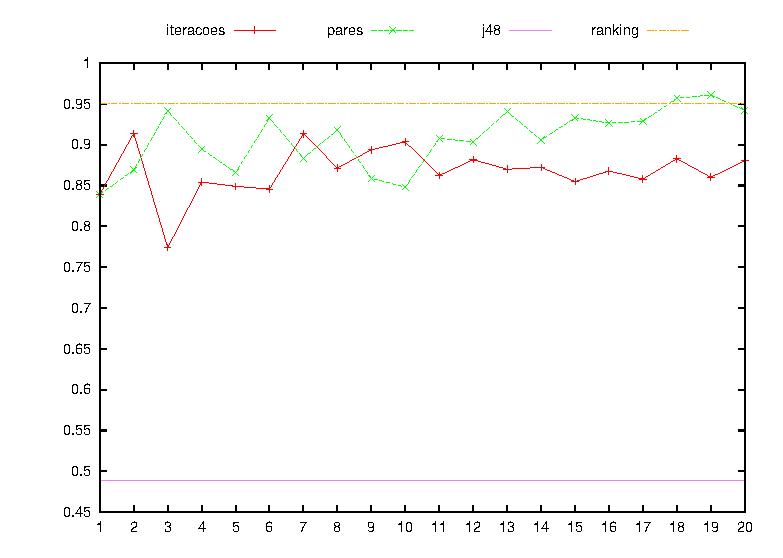
\includegraphics[width=0.9\textwidth]{img/yeast_j48.eps}
        \caption{Gráfico de desempenho para a base Yeast}
    \end{figure}
\end{frame}

\begin{frame}
    \frametitle{Desempenho (AUC): Naïve Bayes (bayes.NaiveBayes)}

    \begin{figure}[H]
        \centering
        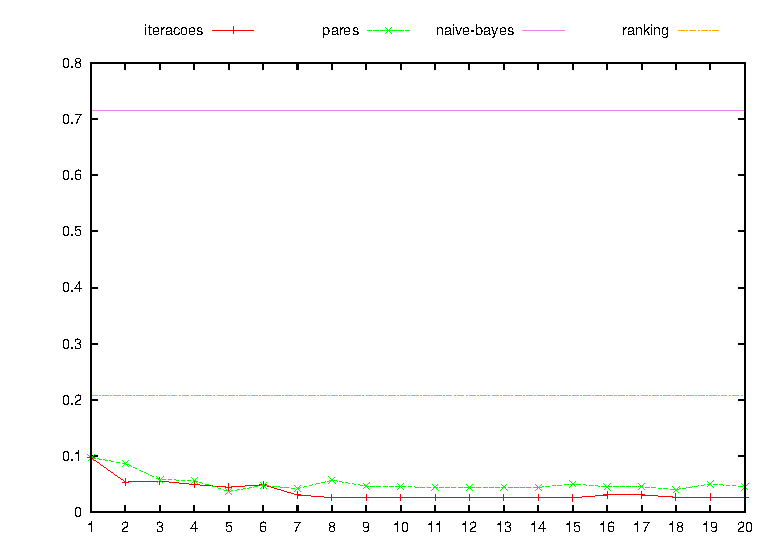
\includegraphics[width=0.9\textwidth]{img/breast-cancer_naive-bayes.eps}
        \caption{Gráfico de desempenho para a base Breast Cancer}
    \end{figure}
\end{frame}

\begin{frame}
    \frametitle{Desempenho (AUC): Naïve Bayes (bayes.NaiveBayes)}

    \begin{figure}[H]
        \centering
        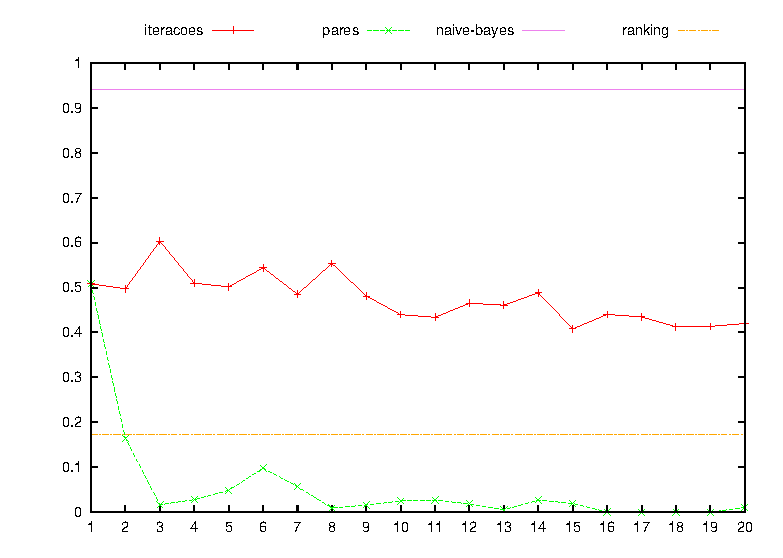
\includegraphics[width=0.9\textwidth]{img/glass_naive-bayes.eps}
        \caption{Gráfico de desempenho para a base Glass}
    \end{figure}
\end{frame}

\begin{frame}
    \frametitle{Desempenho (AUC): Naïve Bayes (bayes.NaiveBayes)}

    \begin{figure}[H]
        \centering
        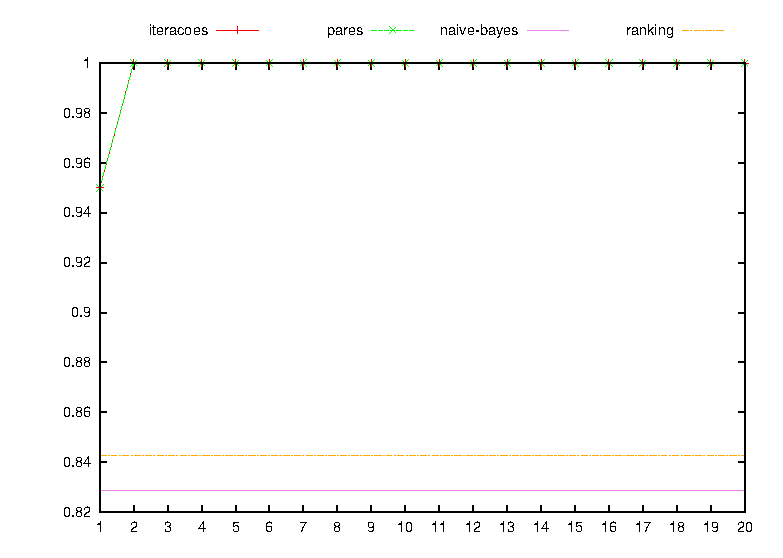
\includegraphics[width=0.9\textwidth]{img/yeast_naive-bayes.eps}
        \caption{Gráfico de desempenho para a base Yeast}
    \end{figure}
\end{frame}

\begin{frame}
    \frametitle{Desempenho (AUC): Curva Logística (functions.Logistic)}

    \begin{figure}[H]
        \centering
        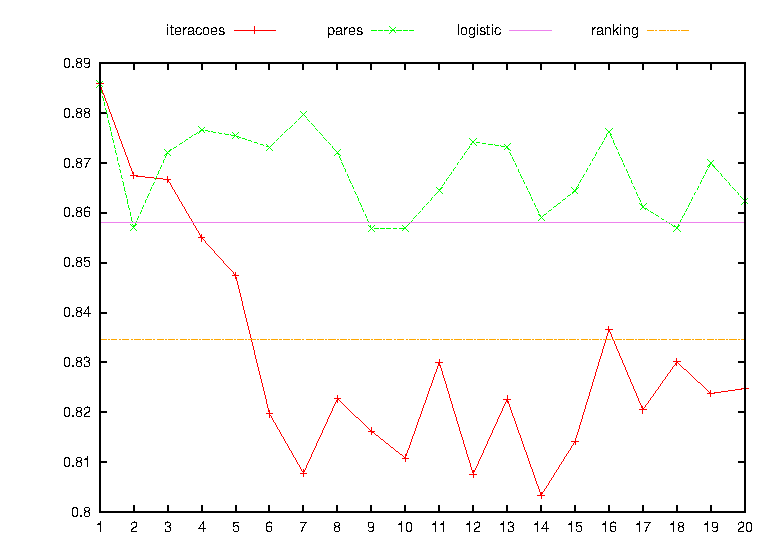
\includegraphics[width=0.9\textwidth]{img/yeast_logistic.eps}
        \caption{Gráfico de desempenho para a base Yeast}
    \end{figure}
\end{frame}

\begin{frame}
    \frametitle{Desempenho (AUC): Support Vector Machine (functions.SMO)}

    \begin{figure}[H]
        \centering
        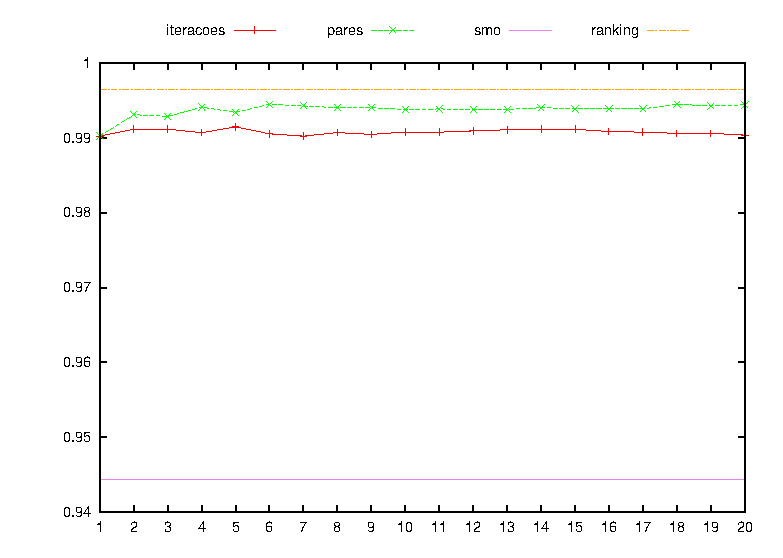
\includegraphics[width=0.9\textwidth]{img/vehicle_smo.eps}
        \caption{Gráficos de desempenho para a base Vehicle}
    \end{figure}
\end{frame}

\begin{frame}
    \frametitle{Desempenho (AUC): Support Vector Machine (functions.SMO)}

    \begin{figure}[H]
        \centering
        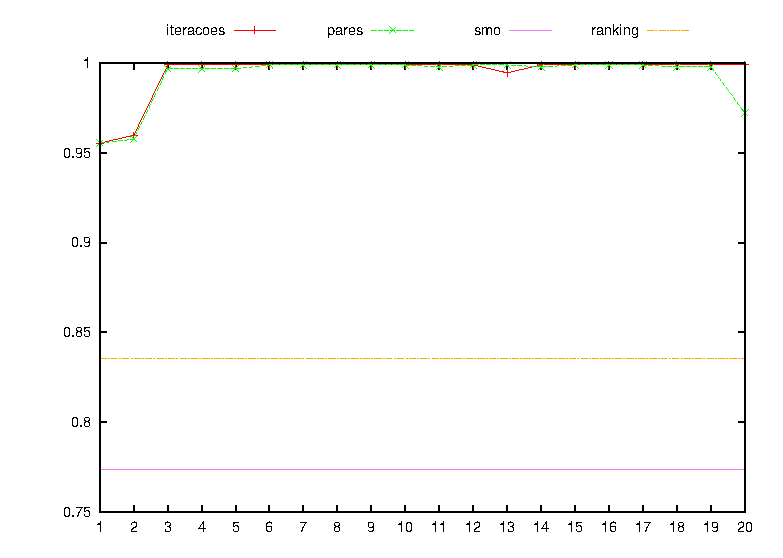
\includegraphics[width=0.9\textwidth]{img/yeast_smo.eps}
        \caption{Gráficos de desempenho para a base Vehicle}
    \end{figure}
\end{frame}